\documentclass{article}
\usepackage[utf8]{inputenc}
\usepackage{lipsum}
\usepackage[margin+1in,incldefoot]{geometry}

\usepackage[hidethelinks]{hyperref} % Allows for double references

% graphics Preamble
\usepackage{graphicx} % Allows to import images
\usepackage{float} % Allows control of float positions
\usepackage{multirow}
\usepackage{multicol}

% Header and footer
\usepackage{fancyhdr}
\pagestyle{fancy}
\fancyfoot{}
\fancyfoot[R]{\thepage}
\renewcommand{\footrulewidth}{1pt}

%
\begin{document}

\begin{titlepage}
    \begin{center}
        \line(1,0){400}\\
        [0.25in]
        \huge{\bfseries Metric Learning Approaches for Face Identification}
        [2mm]
        \line(1,0){400}\\
        [0.25in]
        \textsc{\large Computer Vision (CSE578) Course Project}\\
        [3mm]
        \textsc{\large Akshay Bankar (2019201011) \\
                Angad Yennam (2019900082) } \\
        \textsc{\large April 2020}
    \end{center}

\end{titlepage}

% Table of contents
\tableofcontents
\thispagestyle{empty}
\cleardoublepage
\setcounter{page}{1}

% List of figures
\listoffigures
\addcontentsline{toc}{section}{\numberline{}List of figures}
\cleardoublepage

% List of tables
\listoftables
\addcontentsline{toc}{section}{\numberline{}List of tables}
\cleardoublepage

\section*{Abstract}
\addcontentsline{toc}{section}{\numberline{}Abstract}
\cleardoublepage



\section{Introduction}\label{sec:intro}
\subsection{What is metric learning}
Distance metric learning (or simply, metric learning) aims at automatically constructing task-specific distance metrics from (weakly) supervised data, in a machine learning manner. The learned distance metric can then be used to perform various tasks (e.g., k-NN classification, clustering, information retrieval, data visualization).//

\subsection{Mahalanobis Distances}

Given a real-valued parameter matrix L of shape (num\_dims, n\_features) where n\_features is the number features describing the data, the Mahalanobis distance associated with L is defined as follows:\\
D(x, x') = $\sqrt{{(Lx-Lx')^\top(Lx-Lx')}}$ \\
A Mahalanobis distance is a Euclidean distance after a linear transformation of the feature space defined by L (taking L to be the identity matrix recovers the standard Euclidean distance). Mahalanobis distance metric learning can thus be seen as learning a new embedding space of dimension num\_dims.


\begin{definition}\label{D;metric} Let $X$ be a 
set and
$d:X^{2}\rightarrow{\mathbb R}$ a function with the
following properties:

(i) $d(x,y)\geq 0$ for all $x,\,y\in X$.

(ii) $d(x,y)=0$ if and only if $x=y$.

(iii) $d(x,y)=d(y,x)$ for all $x,\,y\in X$.

(iv) $d(x,y)+d(y,z)\geq d(x,z)$ for all $x,\,y,\,z\in X$.
(This is called the \emph{triangle inequality} after the
result in Euclidean geometry that the sum of the lengths
of two sides of a triangle is at least as great as the
length of the third side.)

Then we say that $d$ is a \emph{metric} on $X$ and that $(X,d)$
is a \emph{metric space}.
\end{definition}
You should imagine the author muttering under his breath

`(i) Distances are always positive.

(ii) Two points are zero distance apart if and only
if they are the same point.

(iii) The distance from $A$ to $B$ is the same
as the distance from $B$ to $A$.

(iv) The distance from $A$ to $B$ via $C$
is at least as great as the distance from $A$ to $B$
directly.'
if a mapping satisfies the first three properties but not the fourth, it is called a
pseudometric.

We obtain a family of metrics over X by computing Euclidean distances after performing a
linear transformation~x′ = L~x. These metrics compute squared distances as:
DL(~xi,~xj) = kL(~xi −~xj)k2 2,

It is common to express squared distances under the metric in Eq. (1) in terms of the square
matrix:
M = L⊤L. (2)
Any matrix M formed in this way from a real-valued matrix L is guaranteed to be positive semidefinite (i.e., to have no negative eigenvalues). In terms of the matrix M, we denote squared distances by
DM(~xi,~xj) = (~xi −~xj)⊤M(~xi −~xj), (3)
and we refer to pseudometrics of this form as Mahalanobis metrics

\newpage
\section{Marginalized K-NN (Mknn)}\label{sec:mknn}
The kNN classification is used to assign single data points xi to one of a fixed set of k classes associated with the training data. The probability of class c for xi is
\begin{figure}[H]
    \centering
    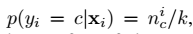
\includegraphics[height=0.7cm]{./mknn_eq1.png}
\end{figure}
where n(i,c) is the number of neighbours of xi of class c.
But the aim here is to predict whether a pair of images (xi, xj) belongs to the same class or not.
To adapt to such clustering marginal probability is computed that assigns xi and xj to the same class using a kNN classifier, which is given by,
\begin{figure}[H]
    \centering
    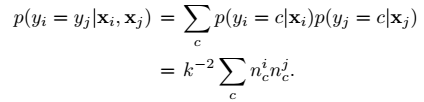
\includegraphics[height=2cm]{./mknn_eq2.png}
\end{figure}
The method can be viewed as a nearest neighbor classifier in the implicit binary labelled
set of $N^2$ pairs. In this set, we need a measure to define neighbours of a pair which can be done by taking all pairs of k neighbours of xi with all of the k neighbours of xj.
The probability for the positive class given by this classifier for a pair
is then determined by the number of positive and negative
neighbour pairs.
Hence the score of our Marginalized kNN (MkNN) binary classifier for a pair of images (xi, xj) is based on how many positive neighbour pairs we can form from neighbours of xi and xj. 
\begin{figure}[H]
    \centering
    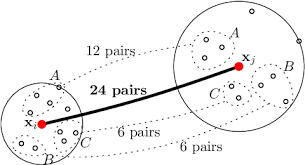
\includegraphics[height=2in]{./mknn_img1.png}
    \caption[M-KNN Schematic Representation]{Schematic representation of k = 10 neighbourhoods for xi and xj, and the 24 neighbour pairs (out of 100) that have the same name and contribute to the score. }
    \label{fig:fig_name}
    
\end{figure}

%%%%%%%%%%%%%%%%%%%%%%%%%%%%%%%%%%%%%%%%%%%%%%%%%%%%%%%%%%%%%%%%%%%%%%%%%%%%%%%%%%%%%%%%%%%%%%%

\section{Large Margin Nearest Neighbor (LMNN)}\label{sec:lmnn}
The method attempts to lean a Mahalanobis distance metric of the form described in above section.
The model has three essential properties : 
(i) Its convex loss function, (ii) its goal of margin maximization, (iii) the constraints on the distance metric imposed by accurate kNN classification.

\subsection{Terminology}
Target neighbors: Each input xi has k nearest neighbors that share its same label yi. These establish a perimeter based on Mahalanobis distance.\\
[0.5cm]
Imposters : These are differently labeled inputs in the training set that invade perimeter set by the target neighbors.
\begin{figure}[H]
    \centering
    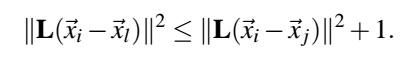
\includegraphics[height=1cm]{./lmnn_eq1.png}
\end{figure}
The model is based on two idealizations: : first, that each training input xi should share the same label yi as its k nearest neighbors (target neighbors); second, that training inputs with different labels(imposters) should be widely separated.

\begin{figure}[H]
    \centering
    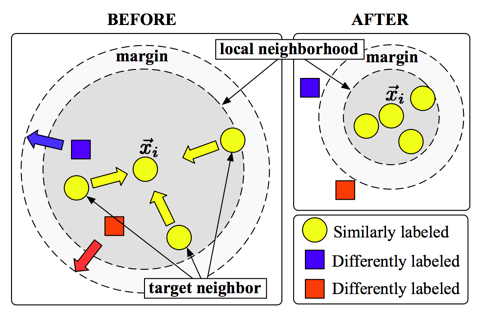
\includegraphics[height=2in]{./lmnn_img1.png}
    \caption[LMNN method working]{Illustration of one input’s neighborhood before training (left) versus after training (right). }
    \label{fig:fig_name}
    
\end{figure}

\subsection{Loss function}
The loss function consists of two terms, one which acts to pull target neighbors closer together, and another which acts to push differently labeled examples further apart.\\
The first term in the loss function penalizes large distances between each input and its target
neighbors.
\begin{figure}[H]
    \centering
    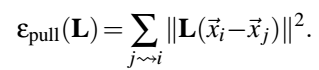
\includegraphics[height=1cm]{./lmnn_eq2.png}
\end{figure}

The second term in the loss function penalizes small distances between differently labeled examples.
\begin{figure}[H]
    \centering
    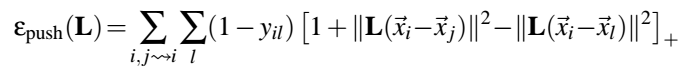
\includegraphics[height=1cm]{./lmnn_eq3.png}
\end{figure}
where the term [z]+ = max(z, 0) denotes the standard hinge loss.

\subsection{Convex optimization}
The loss function defined above is not convex in the matrix elements of the linear transformation L.
To minimize this loss function, approach is prone to being trapped in local minima.\\
This is overcome by reformulating the above equation as an optimization over positive semi-definite matrices.
From section \ref{sec:intro}, D(x, x') denotes the squared distance with respect to the Mahalanobis metric M. Therefore, by substituting for L by D(x, x') in the loss function we get,
\begin{figure}[H]
    \centering
    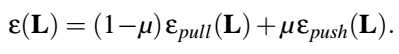
\includegraphics[height=1cm]{./lmnn_eq4.png}
\end{figure}
The loss function is now 
expressed over positive semi-definite matrices M > 0,as opposed to real-valued matrices L. Hence this loss function is a piece-wise linear, convex function of the elements in the matrix M.
\begin{figure}[H]
    \centering
    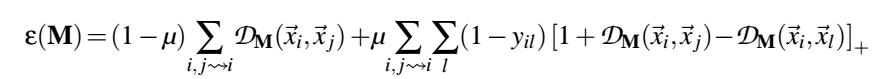
\includegraphics[height=1.2cm]{./lmnn_eq6.png}
\end{figure}
The above optimization can be formulated as an SDP (semi-definite program), which is a linear program that incorporates an additional constraint of that requires the matrix to be positive semi-definite i.e to only have non-negative eigenvalues.
To formulate the above equation as an SDP introduce non-negative slack variables for all triplets of target neighbors ( j~~>i) and impostors xl. The slack variable is used to measure the amount by which the large margin inequality of the imposters is violated. Using the slack variables to monitor these margin violations, the SDP obtained is:
\begin{figure}[H]
    \centering
    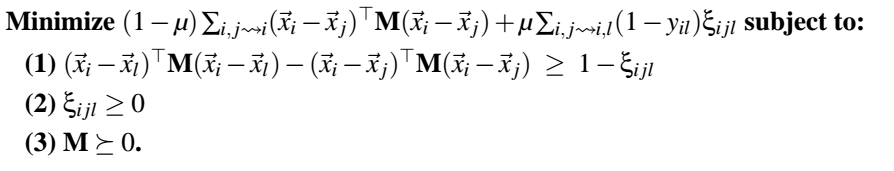
\includegraphics[height=2.5cm]{./lmnn_eq5.png}
\end{figure}
This SDP form can be solved by standard solver packages.

\subsection{Implementation details}
The training images are read and given to face detector module which returns the face ROI. This is done using OpenCV's Face detection implementation which is based on Viola-Jones algorithm. The detected faces are of variable size. These are resized to 150x150.
The resized face images are flattened into 1-D array. On this, dimensionality reduction is performed using PCA such that 95\% of the information is retained.
The reduced eigen faces thus obtained are given to LMNN module which learns the distance metric.
\begin{figure}[H]
    \centering
    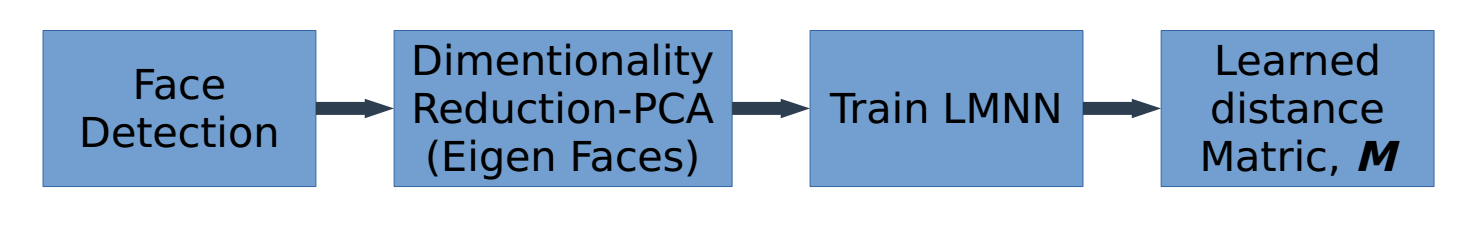
\includegraphics[height=2cm]{./lmnn_img2.png}
\end{figure}

\subsubsection{Parameter setting}
%%%%%%%%%%%%%%%%%%%%%%%%%%%%%%%%%%%%%%%%%%%%%%%%%%%%%%%%%%%%%%%%%%%%%%%%%%%%%%%%%%%%%%%%%%%%%%%

\section{Information Theoretic Metric Learning (ITML)}\label{sec:itml}
An information-theory based distance metric learning algorithm. Given an initial metric, it learns the nearest metric that satisfies some similarity and dissimilarity constraints. The closeness between the metrics is measured using the Kullback-Leibler divergence between the corresponding gaussians.

\subsection{Implementation details}
Refer \ref{sec:ldml_impl} for details which has similar flow.
\subsubsection{Parameter setting}
%%%%%%%%%%%%%%%%%%%%%%%%%%%%%%%%%%%%%%%%%%%%%%%%%%%%%%%%%%%%%%%%%%%%%%%%%%%%%%%%%%%%%%%%%%%%%%%

\section{Logistic Discriminant Metric Learning (LDML)}\label{sec:ldml}
A distance metric learning algorithm that maximizes the likelihood of a logistic based probability distribution.The model is based on the idea that the distance between images in positive pairs to be made smaller than the distances corresponding to negative pairs, and obtain a probabilistic estimation of whether the two images depict the same object.
\subsection{Formulation}
Using the Mahalanobis distance between two images, the method models the probability pn that pair n = (i, j) is positive, i.e. the pair label tn is 1, as:
\begin{figure}[H]
    \centering
        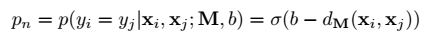
\includegraphics[height=1cm]{./ldml_eq1.png}
\end{figure}
where 
\begin{figure}[H]
    \centering
    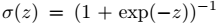
\includegraphics[height=0.6cm]{./ldml_eq2.png}
\end{figure}
is the sigmoid function and b a bias term. The bias works as a threshold value and is learned together with the metric parameters.
Now the probability can be re-written as:
\begin{figure}[H]
    \centering
    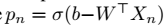
\includegraphics[height=0.7cm]{./ldml_eq3.png}
\end{figure}
where W is the vector containing elements of M and Xn the entries of \(x-x'\).T\(x-x'\).
The parameters of the model are then optimized using the  maximum log-likelihood. The log-likelihood, L, can be written as:
\begin{figure}[H]
    \centering
    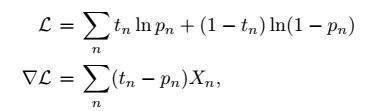
\includegraphics[height=2.5cm]{./ldml_eq4.png}
\end{figure}
This log-likelihood is smooth and concave. Thus, can be solved by gradient ascent.

\subsection{Implementation details}\label{sec:ldml_impl}
The training images are read and given to face detector module which returns the face ROI. This is done using OpenCV's Face detection implementation which is based on Viola-Jones algorithm. The extracted face is the given to shape predictor module which performs 68-point landmark detection. This uses module in Dlib which is implementation of a random forest classifier proposed by Kazimi et al for face landmark detection.
Once the landmark points are obtained, 9 of these points corresponding to eye, nose and lip corners are selected as keypoints for SIFT feature extraction. Corresponding to each point, we get 128-length feature vector at three scales. Thus, for a face image we obtain a 128x9x3 = 3496-length feature vector.
Dimensionality reduction of these feature vectors of train set is performed with number of components equal to 35 as proposed in the paper.
This reduced feature vectors obtained are given to LDML/ITML module which learns the distance metric.
\begin{figure}[H]
    \centering
    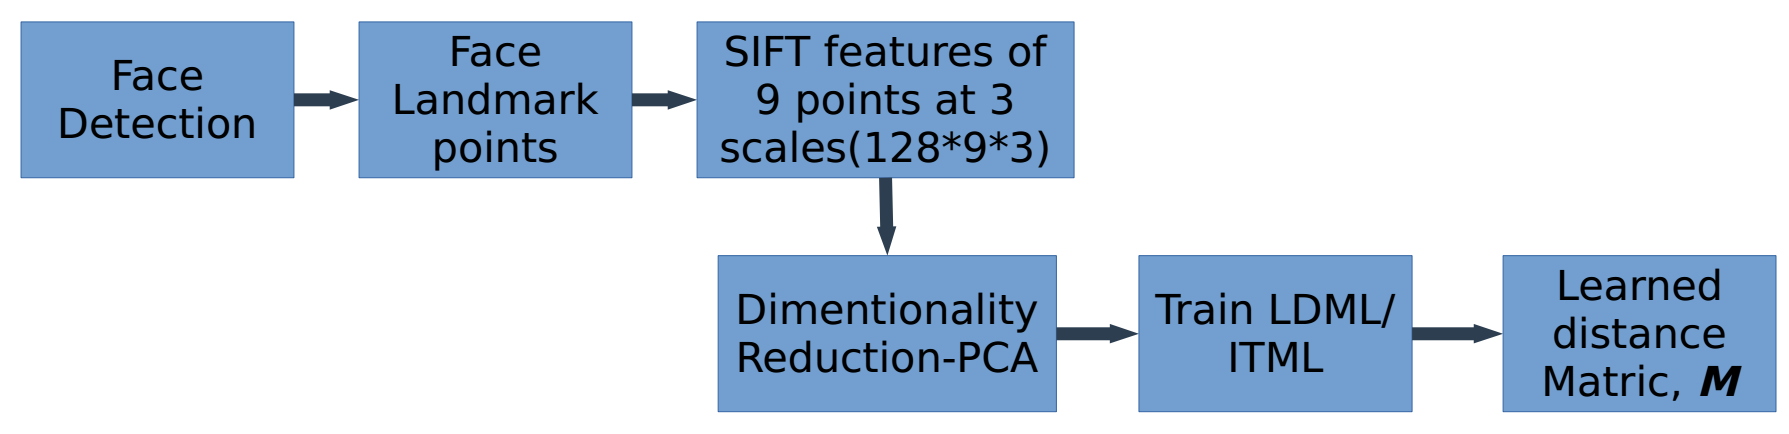
\includegraphics[height=3cm]{./ldml_img1.png}
\end{figure}

\subsubsection{Parameters setting}
%%%%%%%%%%%%%%%%%%%%%%%%%%%%%%%%%%%%%%%%%%%%%%%%%%%%%%%%%%%%%%%%%%%%%%%%%%%%%%%%%%%%%%%%%%%%%%%

\section{Results}\label{sec:results}

\subsection{Dataset}

The Olivetti faces dataset : The dataset contains ten different images of each of 40 distinct subjects. Relatively simpler dataset as the variation is mostly in the lighting and facial expressions.\\
[0.5cm]
Labelled Faces in Wild (LFW) : This dataset is a collection of JPEG pictures of famous people collected over the internet. There are a total of 13233 images and 5749 people in the database.
Each image is a 250x250 jpg. 

\subsection{Performance measure}
The results are reported based on the operating points of the ROC curves.\\
[0.5cm]
AUC-ROC curve : It is a performance measurement for classification problem. ROC is a probability curve and AUC represents degree or measure of separability i.e it tells how much model is capable of distinguishing between classes. The ROC curve is plotted with true positive rate (TPR) against the false positive rate (FPR).

\subsection{Results}
\subsubsection{Performance on Olivetti faces dataset}


\begin{table}[H]
    \centering
    \begin{tabular}{|*{6}{c|}}
    \hline
    \multicolumn{1}{|c}{Method} & \multicolumn{1}{|c|}{NN-method} & \multicolumn{4}{|c|}{ROC classification results} \\ \hline
    \multicolumn{1}{|c|}{} & \multicolumn{1}{|c|}{} & 3-NN & 5-NN & 7-NN & 10-NN \\ \hline
    \multirow{2}{*}{LMNN} & K-NN & 85.28 & 81.45 & 81.47 & 74.14 \\ \cline{2-6}
    & M-KNN & 86.38 & 92.47 & 94.69 & 92.94 \\ \hline
    \multirow{2}{*}{ITML} & K-NN & 89.11 & 90.41 & 87.23 & 89.28 \\ \cline{2-6}
    & M-KNN & 95.20 & 96.31 & 97.14 & 96.20 \\ \hline
    \multirow{2}{*}{LDML} & K-NN & 82.39 & 72.85 & 71.83 & 70.15 \\ \cline{2-6}
    & M-KNN & 96.20 & 95.85 & 96.21 & 94.43 \\ \hline
    \end{tabular}
    \caption{ROC classification result comparison of LMNN, ITML and LDML on Olivetti faces dataset}
    \label{tab:my_label}
\end{table}

\begin{figure}[H]
    \centering
    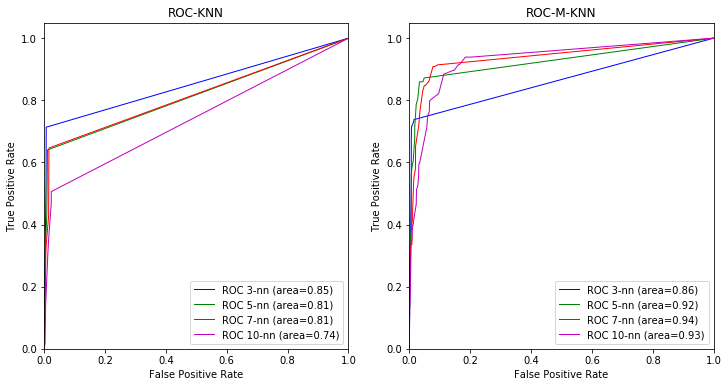
\includegraphics[height=3in]{./lmnn_olv_result.png}
    \caption[LMNN: ROC on Olivetti faces dataset]{ROC classification curve for LMNN method with KNN and M-KNN}
    \label{fig:fig_name}
\end{figure}

\begin{figure}[H]
    \centering
    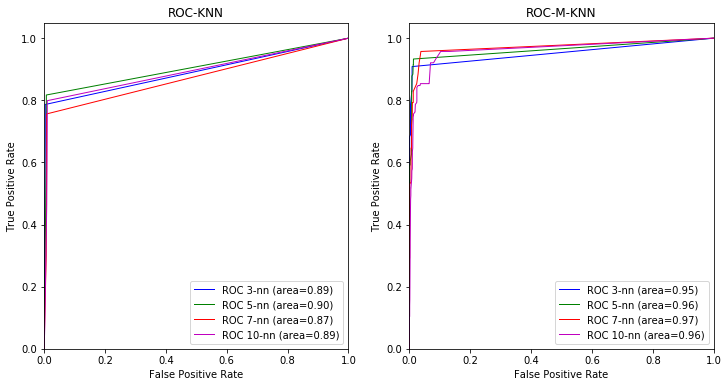
\includegraphics[height=3in]{./itml_olv_result.png}
    \caption[ITML: ROC on Olivetti faces dataset]{ROC classification curve for ITML method with KNN and M-KNN}
    \label{fig:fig_name}
\end{figure}

\begin{figure}[H]
    \centering
    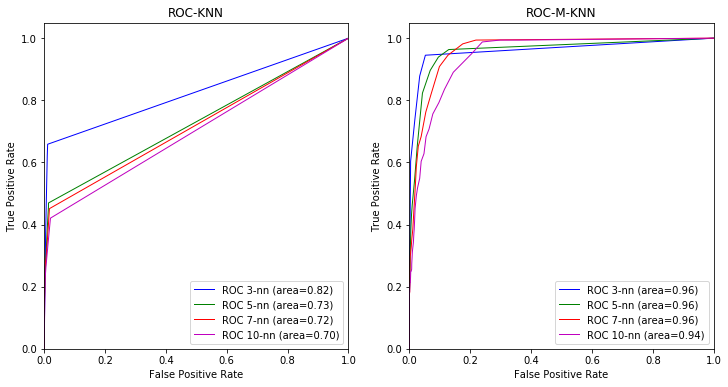
\includegraphics[height=3in]{./ldml_olv_result.png}
    \caption[LDML: ROC on Olivetti faces dataset]{ROC classification curve for LDML method with KNN and M-KNN}
    \label{fig:fig_name}
\end{figure}

\subsubsection{Performance on Labelled Faces in Wild dataset}

\begin{table}[H]
    \centering
    \begin{tabular}{|*{6}{c|}}
    \hline
    \multicolumn{1}{|c}{Method} & \multicolumn{1}{|c|}{NN-method} & \multicolumn{4}{|c|}{ROC classification results} \\ \hline
    \multicolumn{1}{|c|}{} & \multicolumn{1}{|c|}{} & 3-NN & 5-NN & 7-NN & 10-NN \\ \hline
    \multirow{2}{*}{LMNN} & K-NN & 59.01 & 59.23 & 57.23 & 57.70 \\ \cline{2-6}
    & M-KNN & 66.63 & 70.07 & 71.10 & 69.55 \\ \hline
    \multirow{2}{*}{ITML} & K-NN & 59.62 & 62.03 & 62.98 & 65.41 \\ \cline{2-6}
    & M-KNN & 70.48 & 85.38 & 82.65 & 84.10 \\ \hline
    \multirow{2}{*}{LDML} & K-NN & 50.76 & 52.25 & 51.90 & 52.09 \\ \cline{2-6}
    & M-KNN & 60.05 & 62.21 & 60.43 & 67.29 \\ \hline
    \end{tabular}
    \caption{ROC classification result comparison of LMNN, ITML and LDML on LFW dataset}
    \label{tab:my_label}
\end{table}

\begin{figure}[H]
    \centering
    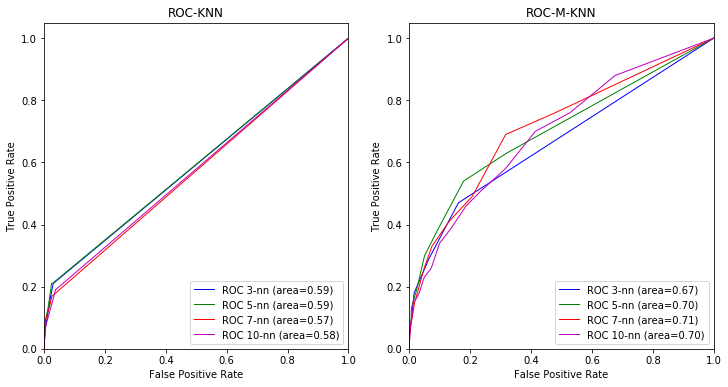
\includegraphics[height=3in]{./lmnn_lfw_result.png}
    \caption[LMNN: ROC on LFW dataset]{ROC classification curve for LMNN method with KNN and M-KNN}
    \label{fig:fig_name}
\end{figure}

\begin{figure}[H]
    \centering
    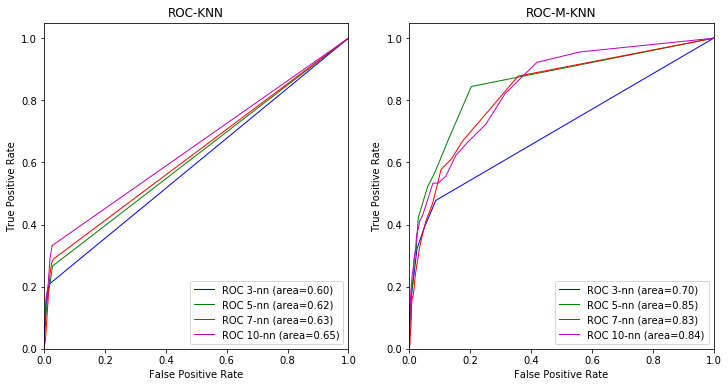
\includegraphics[height=3in]{./itml_lfw_result.png}
    \caption[ITML: ROC on LFW dataset]{ROC classification curve for ITML method with KNN and M-KNN}
    \label{fig:fig_name}
\end{figure}

\begin{figure}[H]
    \centering
    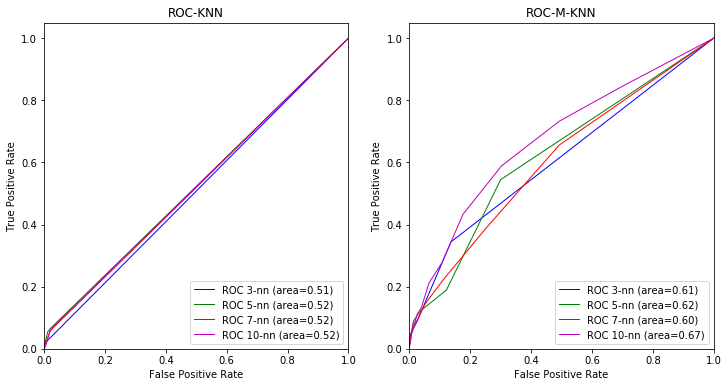
\includegraphics[height=3in]{./ldml_lfw_result.png}
    \caption[LDML: ROC on LFW dataset]{ROC classification curve for LDML method with KNN and M-KNN}
    \label{fig:fig_name}
\end{figure}

%%%%%%%%%%%%%%%%%%%%%%%%%%%%%%%%%%%%%%%%%%%%%%%%%%%%%%%%%%%%%%%%%%%%%%%%%%%%%%%%%%%%%%%%%%%%%%%

\end{document}
